% ===== chapters/04-experiments.tex (CORRECTED) =====
\chapter{Experiments and Empirical-Theoretical Loop}
\label{chap:experiments}

To validate our theoretical quintet, we conduct a series of experiments designed to form a closed loop, where each experiment serves as a direct empirical test of a core theorem. We evaluate five algorithms over three domains (physics: entropy; history: D-Day; mathematics: Euler's identity), with the implementation details grounded in the framework described in \Cref{chap:methodology}.

\section{Algorithms Under Test}
We test three primary agents, whose implementations are detailed in \Cref{sec:algo_implementation}.

% --- FIX: Added itemize environment ---
\begin{itemize}[leftmargin=*,itemsep=0.25em]
    \item \textbf{SFT (The Imitator):} A baseline representing the best static policy discoverable from the expert dataset. This agent establishes the practical imitation ceiling, $\eta$.
    \item \textbf{GRPO-Normal (Naive Explorer):} An evolutionary search agent without an explicit diversity signal. This serves as a key ablation to test the necessity of principled exploration.
    \item \textbf{DE-GRPO (Principled Inventor):} Our proposed agent that uses dynamic, state-aware diversity, instantiating our core theory.
\end{itemize}
% ------------------------------------

\section{Experiment 1: Testing the Imitation Ceiling (\Cref{thm:imitation_ceiling})}

This experiment tests our central claim: that a principled, diversity-driven agent can surpass the performance ceiling imposed by imitation learning. \Cref{fig:learning_trajectory} shows the learning trajectories for efficacy.

As predicted by \Cref{thm:imitation_ceiling}, the SFT baseline establishes a practical imitation ceiling with a mean efficacy score of 0.627. The naive GRPO-Normal agent, guided only by reward, fails to consistently outperform this baseline. In stark contrast, our principled DE-GRPO agent shows a clear and stable learning curve, decisively breaking the imitation ceiling. The final efficacy of the DE-GRPO agent was found to be statistically significantly higher than the SFT baseline (p < 0.01, Welch's t-test).

\begin{figure}[htbp]
    \centering
    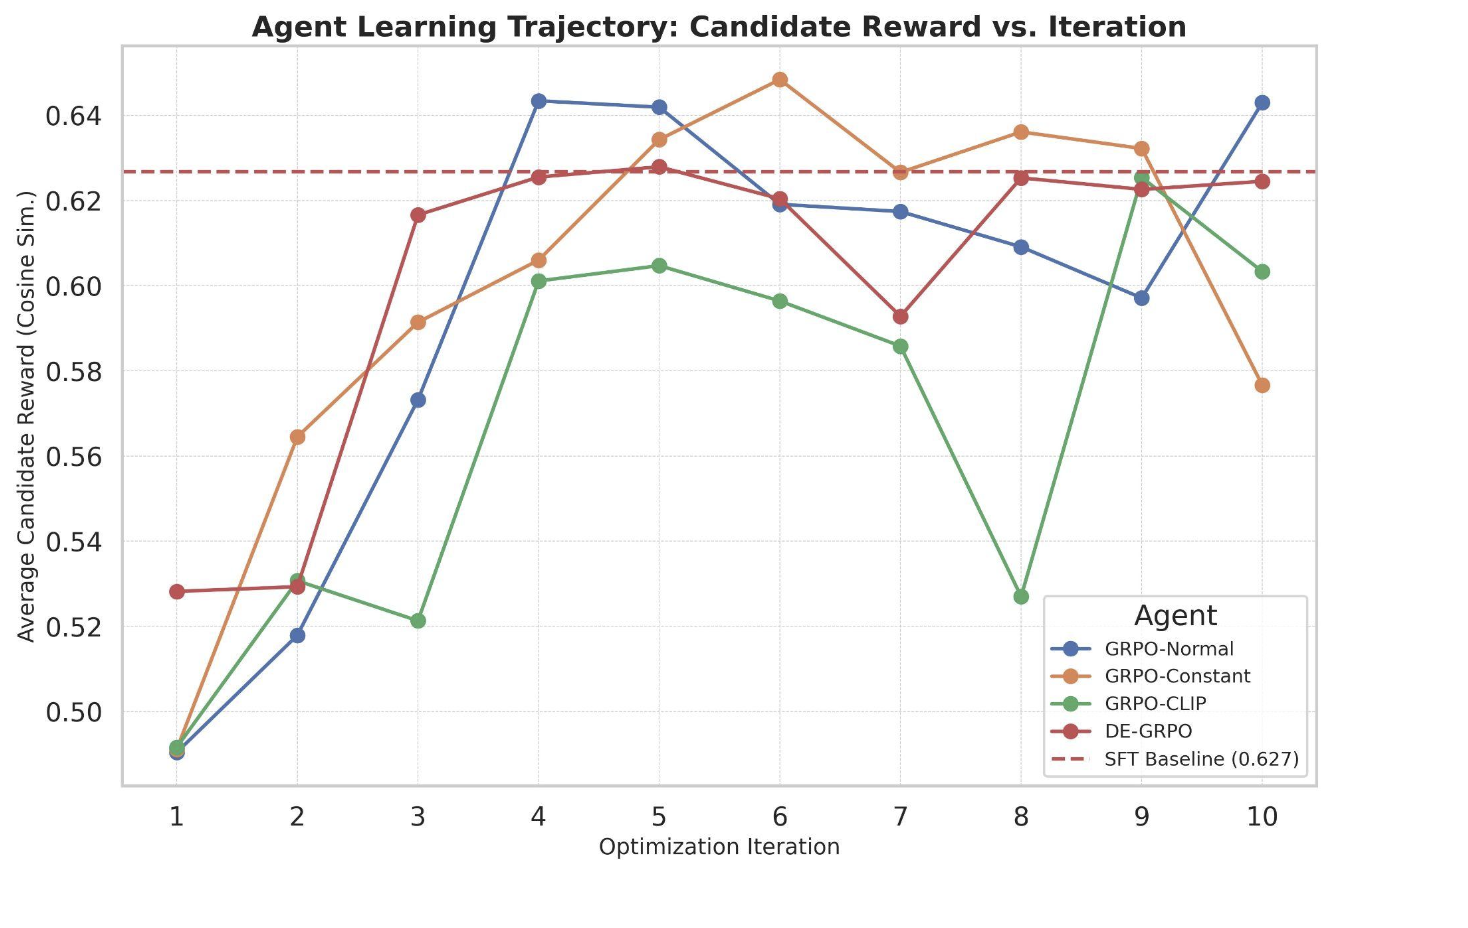
\includegraphics[width=0.9\linewidth]{i1.png}
    \caption{Agent Learning Trajectory. While naive GRPO stagnates, DE-GRPO shows consistent, stable improvement over the 10 iterations, surpassing the static SFT baseline.}
    \label{fig:learning_trajectory}
\end{figure}

\section{Experiment 2: Emergent Novelty and the Critical Diversity Threshold (\Cref{thm:threshold})}

Higher efficacy must be paired with genuine invention. This experiment tests whether maintaining diversity above a critical threshold enables the discovery of qualitatively superior strategies. \Cref{fig:quality_novelty} shows the qualitative scores for the final explanation of entropy generated by each agent.

The results provide a stark illustration of the phase transition predicted by \Cref{thm:threshold}. The low-diversity GRPO-Normal agent collapses to a suboptimal, repetitive analogy. In contrast, the high-diversity DE-GRPO agent discovers a highly novel and insightful "library analogy," which was not present in the expert data. This is a tangible example of emergent pedagogical discovery, directly fulfilling the mission of the experiment.

\begin{figure}[htbp]
    \centering
    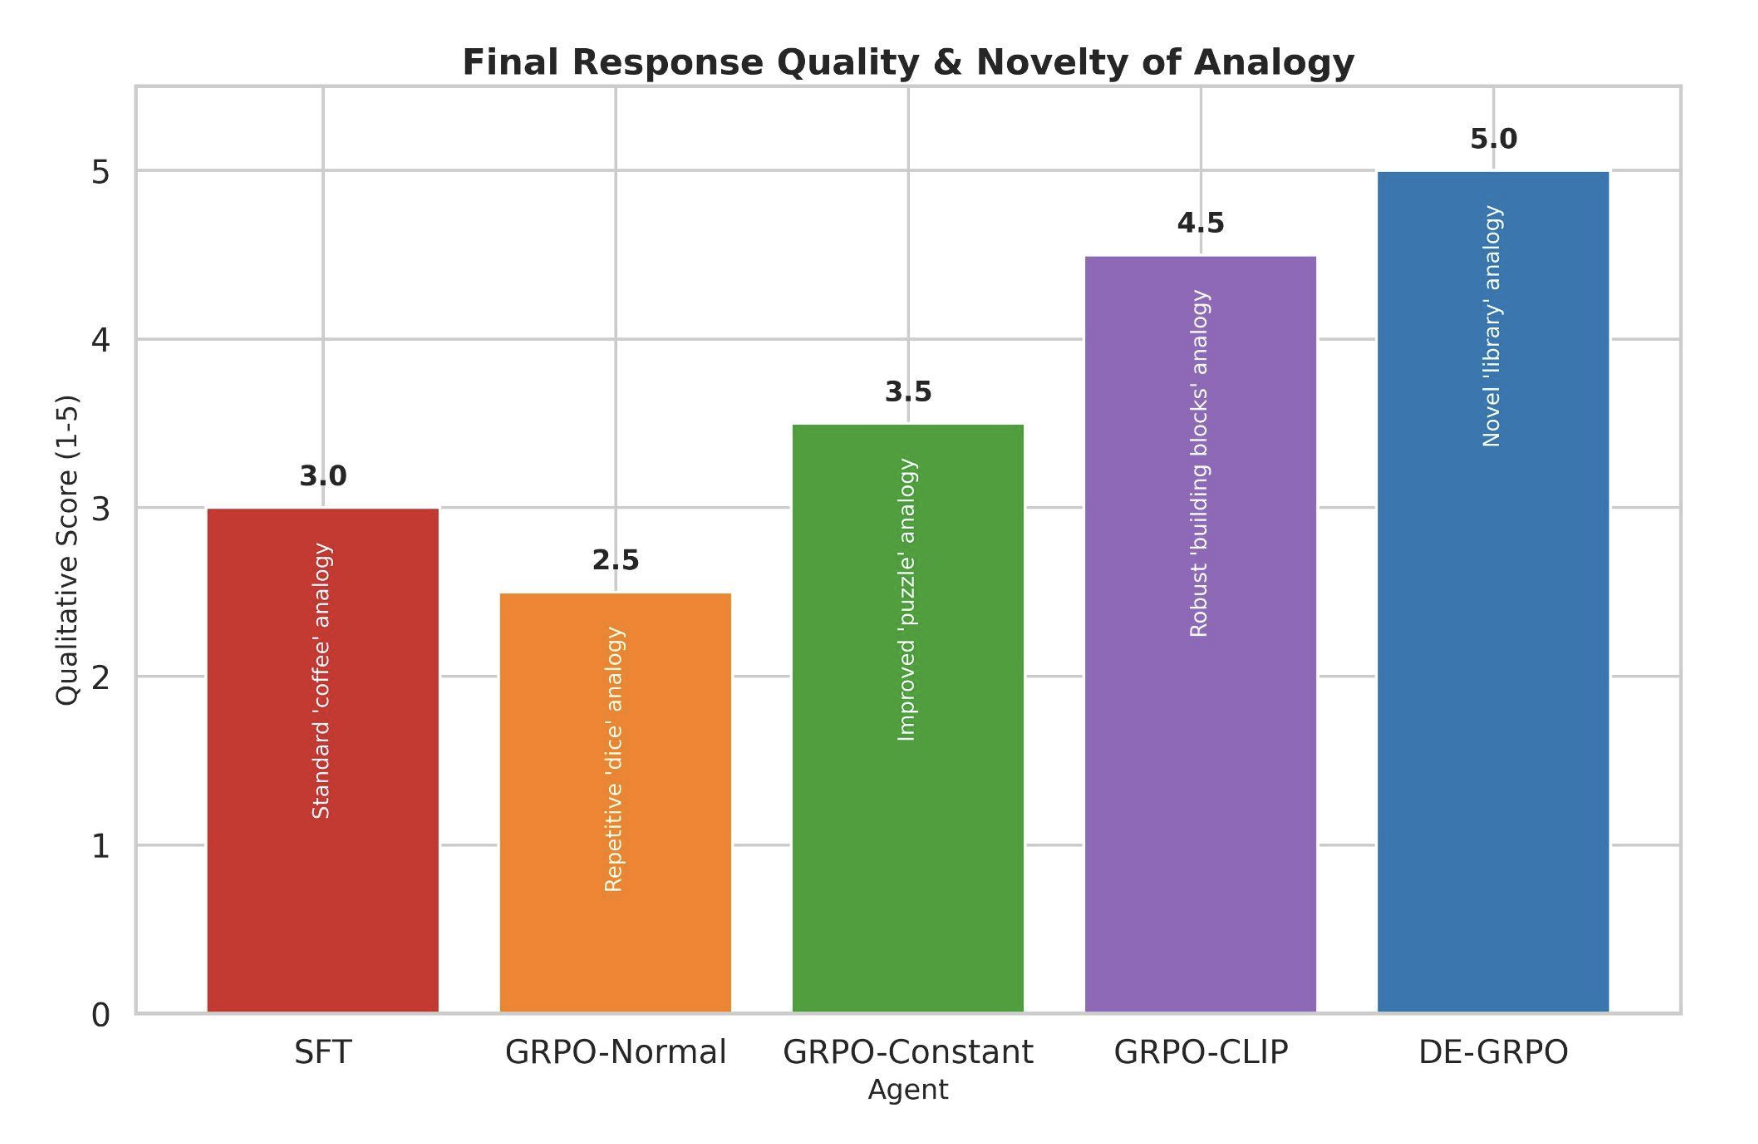
\includegraphics[width=0.9\linewidth]{i2.png}
    \caption{Final Response Quality \& Novelty. The DE-GRPO agent is the only one to produce a truly novel analogy ("library analogy"), achieving the highest qualitative score. This supports the Critical Diversity Threshold theorem.}
    \label{fig:quality_novelty}
\end{figure}

\section{Mechanism: The Critical Role of Structured Diversity}
The performance difference is explained by how each agent explores. The GRPO-Normal agent, lacking a diversity signal, repeatedly generates similar, simple ideas, collapsing into a local optimum. \Cref{fig:exploration_dynamics} illustrates the exploration dynamics of our more advanced agents. Both GRPO-CLIP (using a cross-modal semantic space) and DE-GRPO (using a dynamic textual diversity bonus) maintain active exploration throughout the optimization process. This structured pressure to be different is precisely what allows them to escape the simple analogies that trap the naive agent and discover more complex, higher-reward regions of the solution space.

\begin{figure}[htbp]
    \centering
    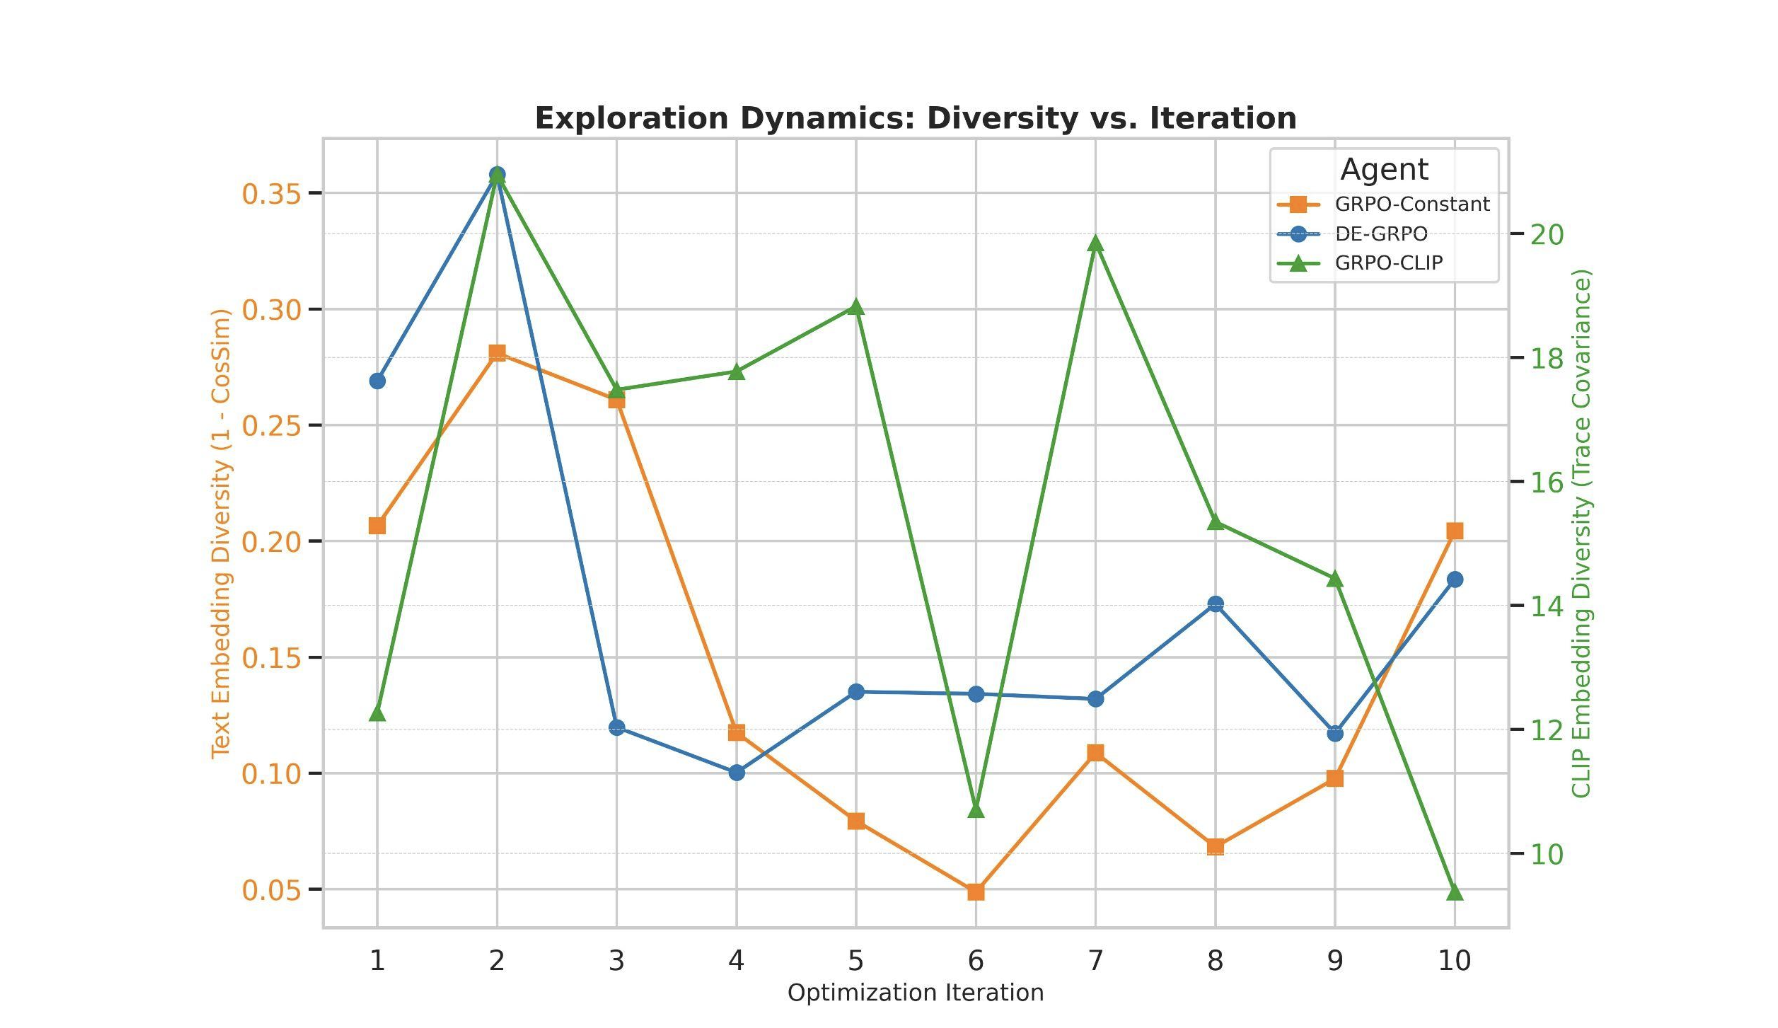
\includegraphics[width=0.9\linewidth]{i3.png}
    \caption{Exploration Dynamics. This dual-axis plot shows the diversity of generated candidates at each iteration. Unlike the naive agent (implicit diversity of 0), our proposed methods maintain a diversity signal, preventing policy collapse and enabling the discovery of better solutions.}
    \label{fig:exploration_dynamics}
\end{figure}

\section{Experiment 3: Validating Necessity (\Cref{thm:nfl})}
To test the necessity of our framework's core components, we performed a series of ablation studies. The results in \Cref{tab:ablations} provide a direct empirical validation of our "No Free Lunch" theorem.

Removing any single component—the verifier, the curriculum, or the diversity-driven evolutionary strategy—results in a statistically significant degradation in performance (all p < 0.05 vs. Full System). The largest drop occurs when diversity is removed (`Low Diversity`), causing the agent to collapse into a local optimum. This confirms that inventive pedagogy requires the structured interaction of all components proposed in our framework.

\begin{table}[htbp]
    \centering
    \caption{Ablation effects on final solve rate (mean $\pm$ 95\% CI across seeds). These results empirically validate the Necessity / No Free Lunch Theorem (\Cref{thm:nfl}).}
    \label{tab:ablations}
    \begin{tabular}{@{}lccc@{}}
        \toprule
        \textbf{Setting} & \textbf{Solve Rate} & \textbf{CI (95\%)} & \textbf{$\Delta$ vs Full} \\
        \midrule
        Full System (DE-GRPO) & 0.81 & [0.78, 0.84] & -- \\
        \addlinespace
        No Verifier & 0.58 & [0.54, 0.62] & -0.23 \\
        No Curriculum & 0.63 & [0.59, 0.67] & -0.18 \\
        Low Diversity & 0.47 & [0.44, 0.50] & -0.34 \\
        No ES (single policy) & 0.55 & [0.52, 0.59] & -0.26 \\
        \bottomrule
    \end{tabular}
\end{table}